% main.tex, to be used with thesis.tex
% This contains the main work of your thesis.

%\bibliography{thesis}  % uses the references stored in Chapter1Radar.bib

\chapter{DSP Data Persistence: Component Design and Architecture}

In order to provide data to users, the RTC scientists use OPeNDAP \cite{opendap}
server to distribute collected data over the Internet. However, this work
proposes the use a KVP database system as described in the previous chapter,
giving options to advanced techniques to scale on data structure and
organization.

This section shows the proposed DSP Data Persistence component for the DSP
Platform as reviewed in chapter 4, as it is responsible for gathering
the DSP Messages sent from any remote DSP instance. First, section 3.1 briefly
describes main events, processes, input and outputs generated by analyzing a
scenario of remote communications between sensors and the DSP Client and
Server nodes. Then, section 3.2 shows the requirements specification based on
the analysis of section 3.1 and the documentation of the DSP Platform of
section 2.4.

\section{Business Process Analysis}

As described in section 2.4, the Data Sensor Platform was designed to support
an environmental sensor network based in San Francisco Bay, composed by
different types of sensors. The process of extracting the measurements from the
sensors to be reused using the DSP Platform can be summarized following the UML
Business Process diagram depicted in figure
\ref{fig:fig:dsp-persistence-business-process}. It is important to note that
this diagrams details remote communication between sensor devices and a
centralized server, as part of the main scenario to solve the problem of data
persistence.

\begin{figure}[!b]
  \centering
  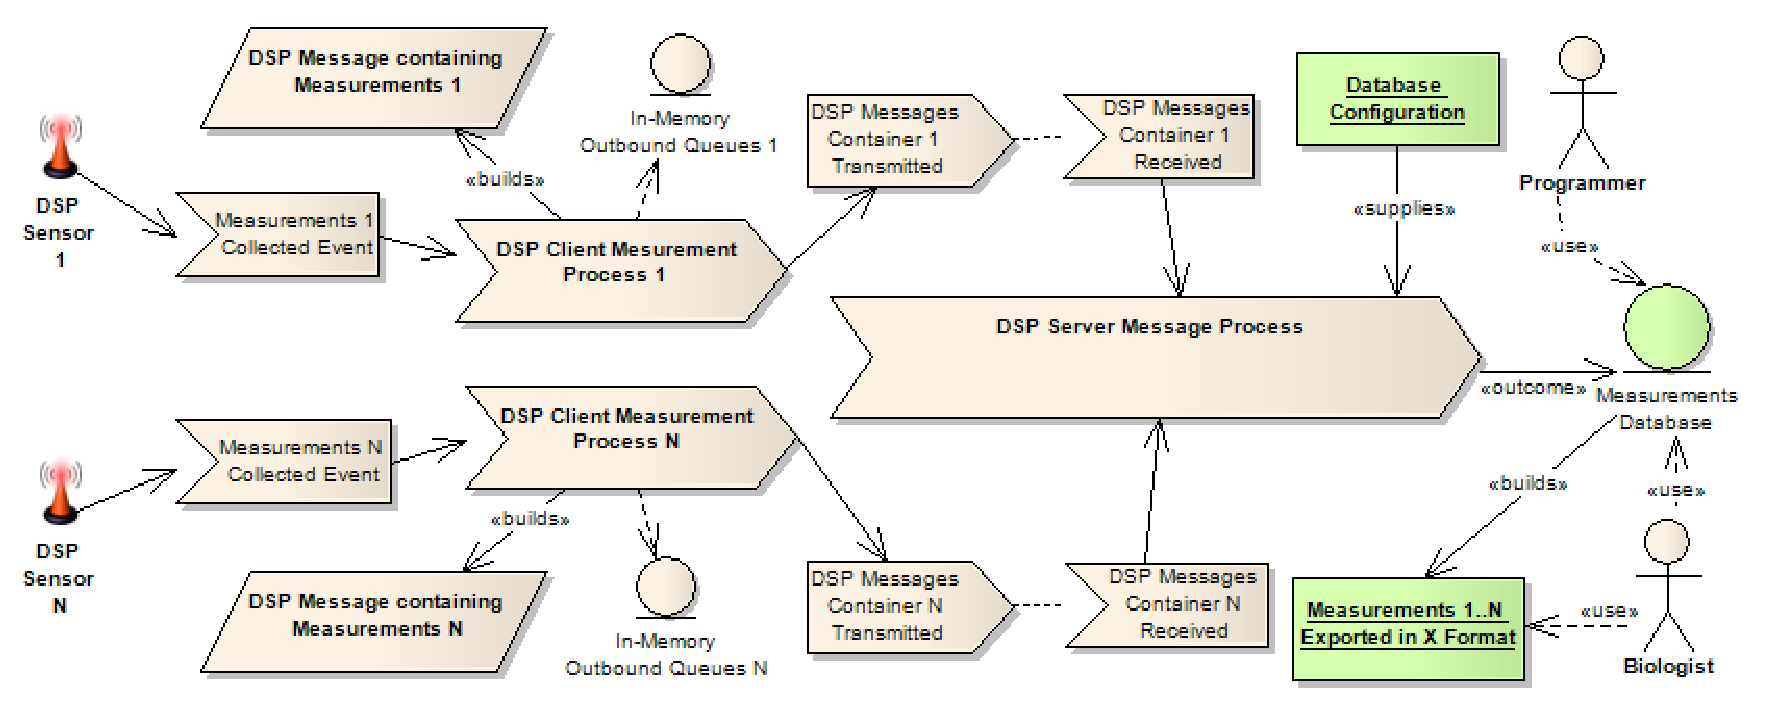
\includegraphics[scale=0.5]{../diagrams/DSP-DataPersistence-Business-Diagram}
  \caption{UML Business Process Model diagram - Adding Persistence for NetBEAMS}
  \label{fig:dsp-persistence-business-process}
\end{figure}

At the event of data collection, the DSP Client receives measurements collected
from each of the sensor devices. Each of the co-located DSP Client processes
the collected measurements and transforms them into the so-called DSP Message
(section 2.4), which embodies the actual data values. After proper data
processing, transformation and categorization, the DSP Message is added into an
in-memory data storage identified (section 2.4). Then, as an asynchronous data
transmission event occurs with an specified rate, transferring all the queued
messages to be processed by a DSP Server host. As it is detailed in image
3.1.1, the server is centralized and is able to concurrently process messages.

This work proposes the addition of a database system that is responsible for
storing the gathered measurement data from sensor hosts on a given network. As
it is shown in image 3.1.1,  the processed measurement data from sensors 1
through N must be collected in the same fashion and categorized as necessary.
In this way, end users such as Biologists and/or Programmers can access the
collected measurements directly from the Database. Furthermore, the same
measurement data is supposed to be exported to different formats as the users
find necessary.

As a matter of fact, the measurements data collected from the sensor devices
are simple  properties with and associated values as described on section 2.1.
According to the descriptions of the DSP Platform and the DSP Messages
structure on section 2.4, the data is represented in programming language
formats such as Java or in a serialized version in XML. Similarly, the
collected data contains measurements that uniquely identifies them, together
with other properties such as time stamps of data creation and collected, as
well as the the IP address of the DSP Client that produced the data. Therefore,
these are important properties for the proposed solution of this work.

\section{Requirements Specification}

By analyzing the main scenario of data process on section 3.1, this section
lists the main use cases that the system and the primary users require. One of
the primary requirements of the system is to enable the use a persistence
system that does not promote the use of specialized professionals to deal with
data modeling, as it is required in most projects using the Structured Query
Language (SQL) [db01], used to extract data from a Relational Database [db01].

\subsection{Functional Requirements}
As part of the user stories related to data access, figure
\ref{fig:DSP-Data-Persistence-UseCases-Diagram-Users} describes the use cases
that the end users can perform with the system.

\begin{figure}[!b]
  \centering
  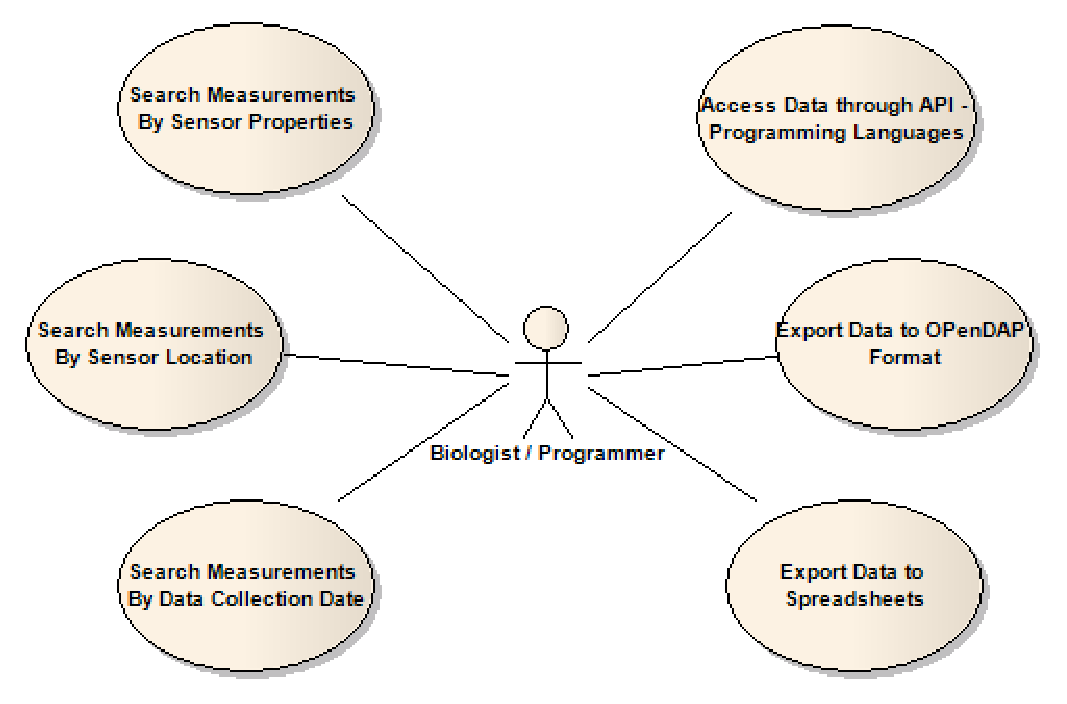
\includegraphics[scale=0.5]{../diagrams/DSP-Data-Persistence-UseCases-Diagram-Users}
  \caption{UML Use Case diagram for Persistence Functions}
  \label{fig:DSP-Data-Persistence-UseCases-Diagram-Users}
\end{figure}

The functional requirements listed in this section are in the format of UML
User Cases [se05]. Figure
\ref{fig:DSP-Data-Persistence-UseCases-Diagram-System} summarizes the use
cases that the system, as the main actor of the system, must perform:

\begin{figure}[!b]
  \centering
  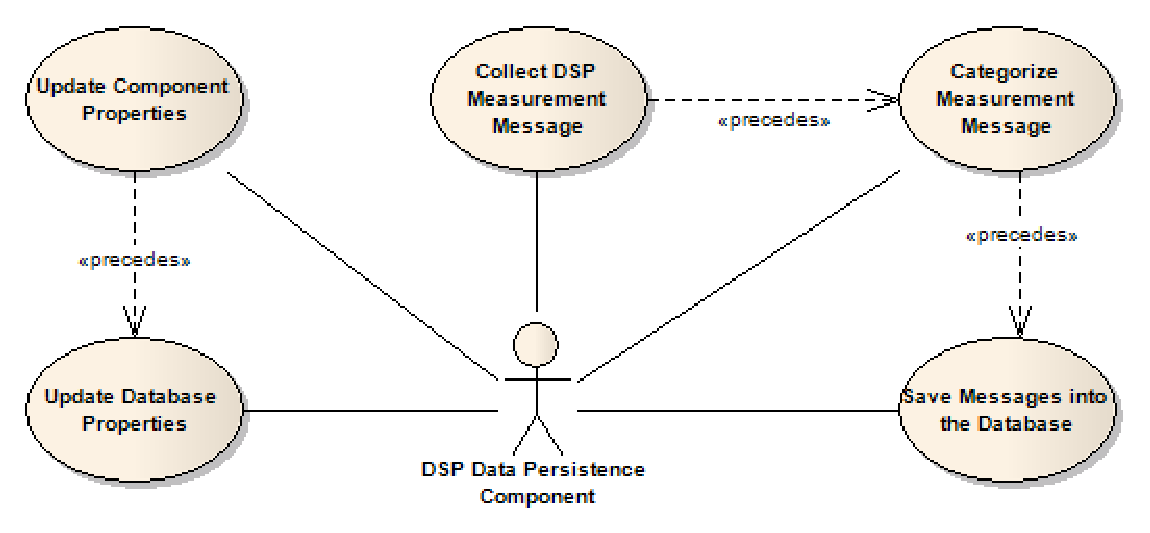
\includegraphics[scale=0.5]{../diagrams/DSP-Data-Persistence-UseCases-Diagram-System}
  \caption{UML Use Case diagram for System Persistence Functions}
  \label{fig:DSP-Data-Persistence-UseCases-Diagram-System}
\end{figure}

\subsection{Non-Functional Requirements}

\begin{itemize}
  \item The DSP Data Persistence component must maintain the received DSP
  Measurement Messages in-memory for a specific rate in order to decrease the
  write load on the database;
  \item The Persistence storage system must be able to cope with dozens of DSP
  Messages;
  \item The Persistence storage system must be able to save measurements quickly;
  \item The Persistence storage system must be able to scale without too much
  architectural changes;
  \item The Persistence storage system must not impose the knowledge of
  complicated database system languages such as SQL [db01] or XML XPath [db05],
  but use access through API calls, since it is closer to researchers. 
\end{itemize}
    
\section{Data Model Design}

After analyzing section 2.1 along with the functional and non-functional
requirements described on section 3.2.2, this work considered the
Key-Value-Pair Data model as described on Section 2.5. Taking into account the
mongoDB architecture and the properties of a DSP Message (see section
"Acquiring the properties of a DSP Message Content" at DSPDataPersistence),
here are the conventions followed on revision r585. The following is the list
of properties that composes the Key of a document:

\begin{itemize}
  \item \textbf{sensor\underline{ }ip\underline{ }address}: it's extracted from
  the DSP Message Produce and identifies which sensor generated the sampling;
  \item \textbf{message\underline{ }id}: it's extracted from each of the messages contained
  in the DSP Message Container;
  \item \textbf{transaction\underline{ }time}: it's extracted from the DSP message container
  creation time and it is used to identify when the transaction occurred (see Section 2.2);
  \item \textbf{fact\underline{ }time}: it's extracted from the SondeDataContainer's date
  and time, and identifies the time in which the collected data occurred (see Section 2.2);
  \item \textbf{latitude}: the latitude variable of the position;
  \item \textbf{longitude}: the longitude variable of the position.
\end{itemize}

The definition of the Value of a document is as follows:

\begin{itemize}
  \item data: this key defines the values of the document, and will have every
  different property of the sensor (see Section 2.4):
   \begin{itemize}
     \item battery
     \item temperature
     \item salinity
     \item \ldots
   \end{itemize}
\end{itemize}

Some remarks about the creation of the items contained with the collections. In
case a message container contains multiple readings in a message container,
each item will be counted as individual snapshots of the data. Also, it is
important to note that the description of the data follows no pattern other
than the description of the properties of the sensor device. However, some
studies have shown that when disk space maximization is required, the name of
database columns are important.

\section{High-Level System Architecture}

Considering the business analysis described in section 3.1, the addition of a
data persistence layer to the DSP Platform can be achieved by adding Data
Consumer (DC) as described in section 2.4. Based on the Requirements
specification described in section 3.2, this component must be responsible for
providing the processing of the DSP Measure Messages into Database-ready
representation, as well as providing the necessary tools for the transmission
of the data to a database system. Figure
\ref{fig:NetBEAMS-Persistence-Server-Node-Components} provides an
architectural view of the DSP Server node with the loosely-coupled components,
highlighting the inclusion of the DSP Data Persistence.

\begin{figure}[!b]
  \centering
  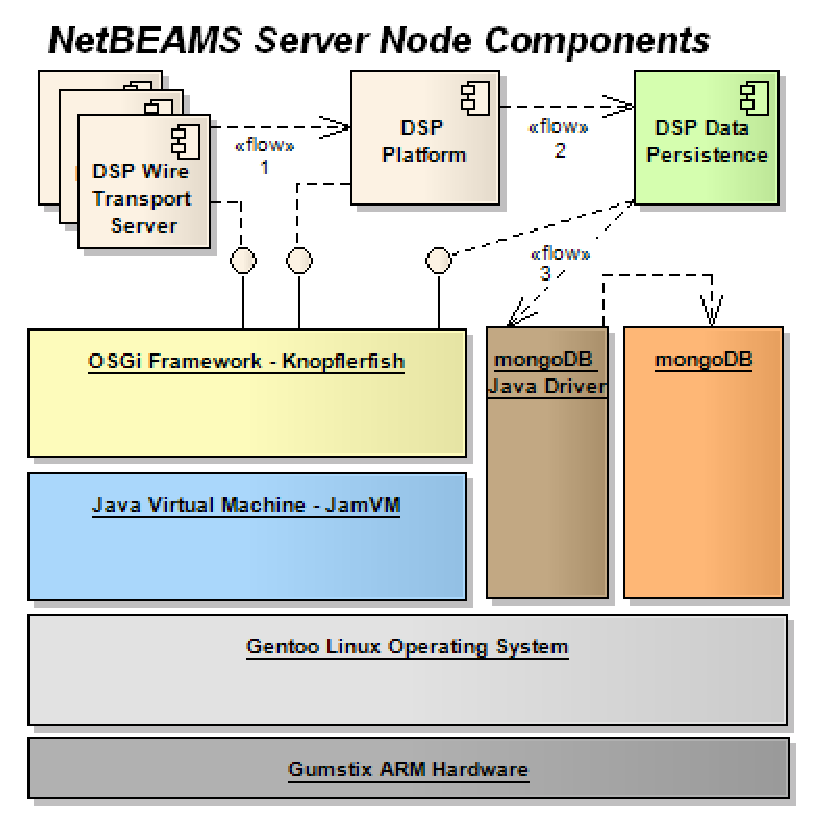
\includegraphics[scale=0.5]{../diagrams/NetBEAMS-Persistence-Server-Node-Components}
  \caption{UML Components diagram of the DSP Data Collector}
  \label{fig:NetBEAMS-Persistence-Server-Node-Components}
\end{figure}

As it is depicted on image 3.4.1, the DSP Data Persistence component can be
added into the system as an independent plug-and-play component. In addition,
the database system and the necessary drivers are also added without any
changes to the existing DSP infrastructure. First, as DSP Messages are
delivered to the server through the DSP Wire Transport Server, as shown by flow
1, the DSP Platform is responsible to forward a copy of the Measurement
messages directly to the DSP Data Persistence as shown by flow 2. Then, the
sole responsibility of the DSP Data Persistence is to transfer the received
measurement messages to the database system by using the connection drivers, as
depicted by flow 3.

The following sections focus on the DSP Data Persistence component design, and
in this way, any references to the DSP Platform can be seen on section 2.4.

\section{DSP Data Persistence: OSGi-DSP Bundle Design}

The new proposed Data Persistence component must follow the DSP requirements
for a new DSP Component. As described on section 2.4, any DSP component follows
the design-pattern of Data Producer/Consumer. Similarly, section 3.2 described
the requirements that the DSP Data Persistence must handle, taking into account
the data model and database connection.

After reviewing the requirements of section 3.2, the resulting model maintains
the dependency among 4 different major Java packages. The addition of a DSP
Data Persistence component depends on 2 existing packages, namely the OSGi
Framework and the DSP Platform as in any DSP Component, and an additional
package for the database access driver API. The UML Package dependency diagram
of image 3.5.x shows these dependencies, which are used to better track changes
among the packages.

\begin{figure}[!h]
  \centering
  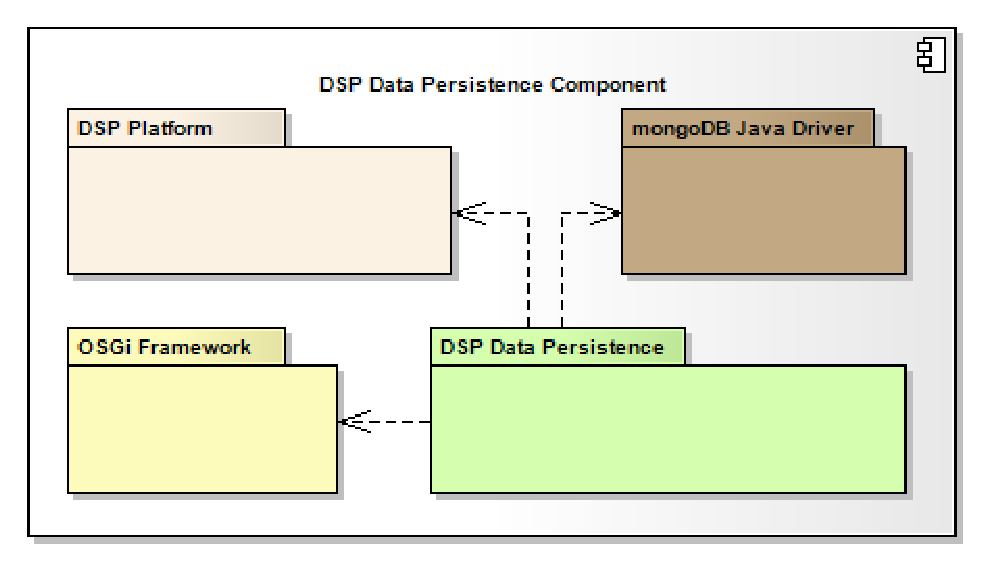
\includegraphics[scale=0.5]{../diagrams/DSP-Data-Persistence-Packages-Dependency}
  \caption{UML Components diagram of the DSP Data Collector}
  \label{fig:DSP-Data-Persistence-Packages-Dependency}
\end{figure}

The following sections details each step of the DSP Data Persistence activation
and parallel execution of the contained classes.

\subsection{DSP Data Persistence Activation and Message Delivery}

As shown on section 2.4.3, the DSP Platform is composed of loosely-coupled
components. In this way, this section describes the addition of the DSP Data
Persistence, as shown on the UML Class diagram of image 3.5.1.1.

\begin{figure}[!h]
  \centering
  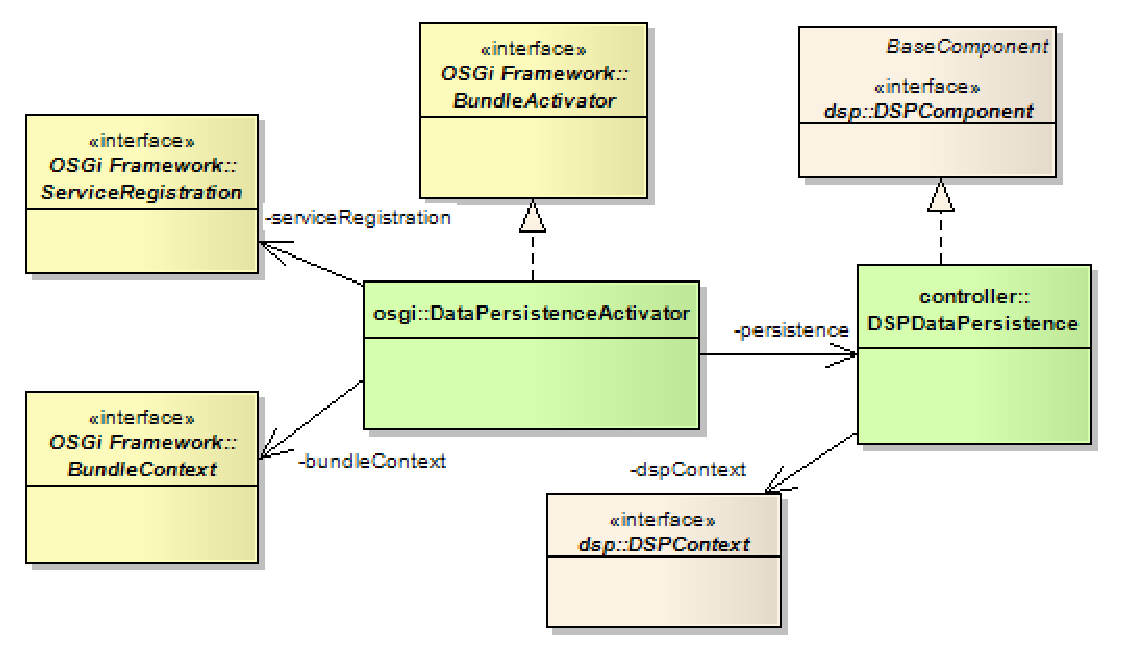
\includegraphics[scale=0.5]{../diagrams/DSP-DataPersistence-Activator-Class-Diagram}
  \caption{UML Class diagram for the DSP Data Persistence Activator and Component}
  \label{fig:DSP-DataPersistence-Activator-Class-Diagram}
\end{figure}

The DSP Data Persistence Activator is the main class responsible for the
activation of the DSP Data Persistence component, as it extends the OSGi class
BundleActivator and maintains a reference of the DSP Data Persistence class.
Furthermore, the activator maintains references to the classes BundleContext
and ServiceReference both from the OSGi Framework. The former is responsible
for maintaining the link with the OSGi Framework, while the latter is used to
register the DSP Component as a service. Therefore, it is clear that the class
DSP Data Persistence Activator is the main communication interface between the
DSP Platform and the OSGi Framework.

While the DSP Data Persistence Activator is responsible for the orchestration
of the classes during the execution on the OSGi Framework, the class DSP Data
Persistence extends from the DSP Platform class DSPComponent. For this reason,
this class inherits all the behavior described on section 2.4 and can be in the
roles of Data Consumer and a Data Producer.

\begin{itemize}
  \item \textbf{DSP Data Persistence as Data Consumer}: receives any measurement
  message from remote sensors;
  \item \textbf{DSP Data Persistence as Data Producer}: transforms any
  measurement message received into a format that must be ready to be saved on the
  database, based on the description of the data model of section 3.3.
\end{itemize}

The DSP Data Persistence Activator follows the states described on the state
diagram of image 2.4.3.4, as it is an extension of the OSGI class
BundleActivator, as well as being responsible for stopping or starting the the
DSP Data Persistence component instance. As described on section 2.4, the
following steps must take place in order to activate and start the DSP Data
Persistence component, described partially on image 2.4.6.3:

\begin{enumerate}
  \item During the DSP Platform activation, it will get the name of the
  persistence component from the configuration artifact config.xml;
  \item After being selected based on the configuration priority, the DSP
  Bundle artifact is identified and installed, by creating an instance of the
  class DSP DataPersistence Activator and making a call to the method start(),
  as shown on image 3.5.1.2;
  \item During the activation, an instance of the DSP Data Persistence
  component is created and registered as an OSGi Service;
  \item Upon registering the DSP Data Persistence component, the DSP Platform
  "listens" the event serviceUpdate() and, and triggers the last operations to
  bootstrap the DSP Component:
   \begin{enumerate}
      \item Initializes the component by calling the method initComponent();
      \item Starts the component by calling the method startComponent();
      \item Bootstrap messages are delivered to the component.
   \end{enumerate}
\end{enumerate}

As the requirements defined on section 3.2 specifies the update of the DSP
Component during its initialization, an optional DSP Update Message will be
sent to the component during its initialization process, as described on
section 2.4. The initialization of the DSP Component Activator and the DSP
Component registration are shown on image 3.5.1.2.

\begin{figure}[!b]
  \centering
  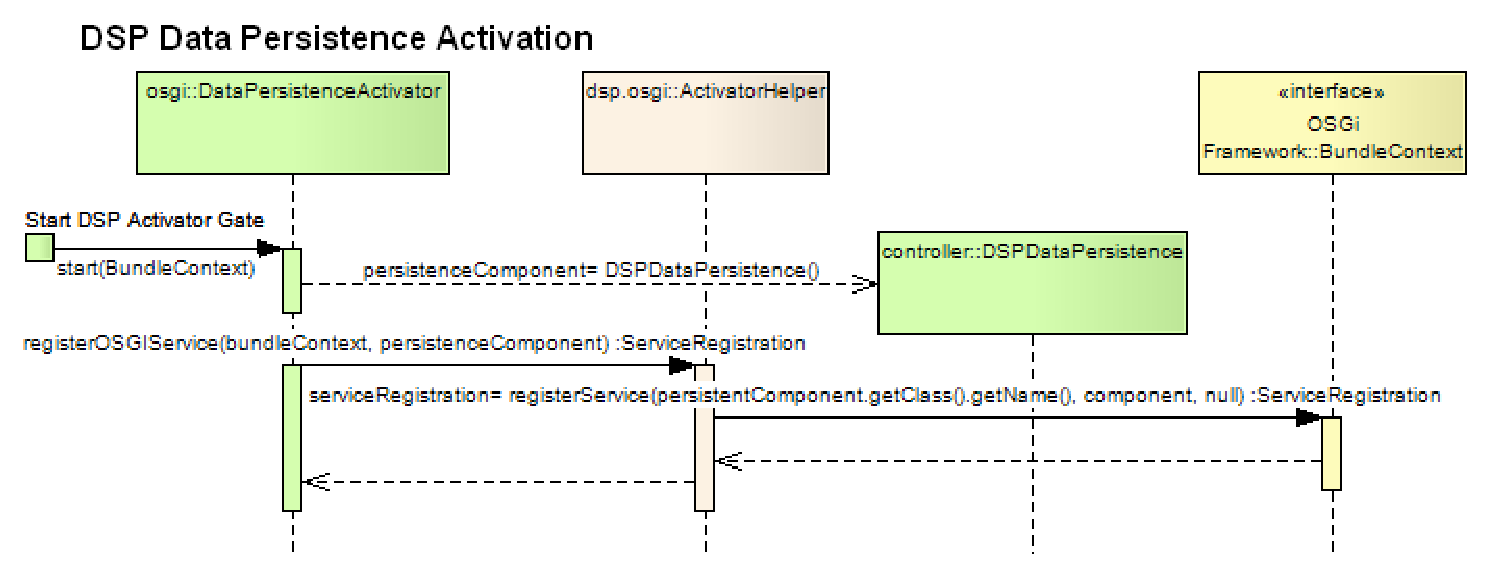
\includegraphics[scale=0.5]{../diagrams/From-OSGi-Framework-to-DSP-Data-PersistenceActivator-Sequence-Diagram}
  \caption{UML Sequence diagram describing the DSP Data Persistence bundle activation}
  \label{fig:From-OSGi-Framework-to-DSP-Data-PersistenceActivator-Sequence-Diagram}
\end{figure}

The the gate "Start DSP Activator Gate" reaches the DSP Data Persistence, it
first creates the unique instance of the class DSP Data Persisence and uses
that instance to register it as the OSGi service through the call to the DSP
Platform helper class ActivatorHelper. At this point, the DSP Data Persistence
has been installed and is in the state "Active".

\subsection{Delivering Bootstrap and Measurement Messages}

Although the DSP Data Persistence component has been instantiated as of image
3.5.1.2, the process of delivering messages to the DSP Data Persistence has yet
to be completed. As defined by the requirements, the DSP Component must execute
its function in a concurrent fashion, using configuration parameters during its
bootstrap process. The class DSP Data Flusher is responsible for running as a
"worker thread", whose function is to verify if there are messages to be
flushed into the Database with the class Transient Persistence Layer. Image
3.5.2.1 describes the remaining UML Class diagram for the main classes of this
functionality.

\begin{figure}[!b]
  \centering
  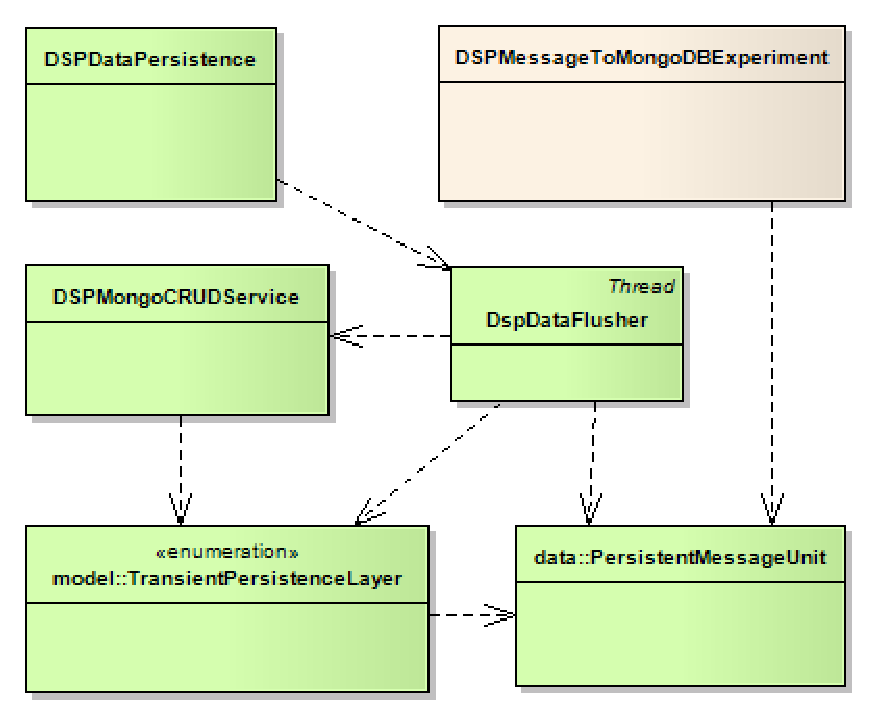
\includegraphics[scale=0.5]{../diagrams/DSP-DataPersistence-Flusher-Classes}
  \caption{UML Class diagram with the DSP Data Flusher worker thread}
  \label{fig:DSP-DataPersistence-Flusher-Classes}
\end{figure}

The DSP Data Flusher is a thread that is designed to be in two different
states: RUNNABLE and TIMED\underline{ }WAITING. In the former, the DSP Data Flusher will be
contacting the Transient Persistence Layer to verify if there are any message
waiting to be sent to the Database service, while in the latter the DSP Data
flusher will be waiting for the next cycle defined by the bootstrap parameter
TRANSIENT\underline{ }DATA\underline{ }FLUSHER\underline{ }DELAY.


\begin{figure}[!b]
  \centering
  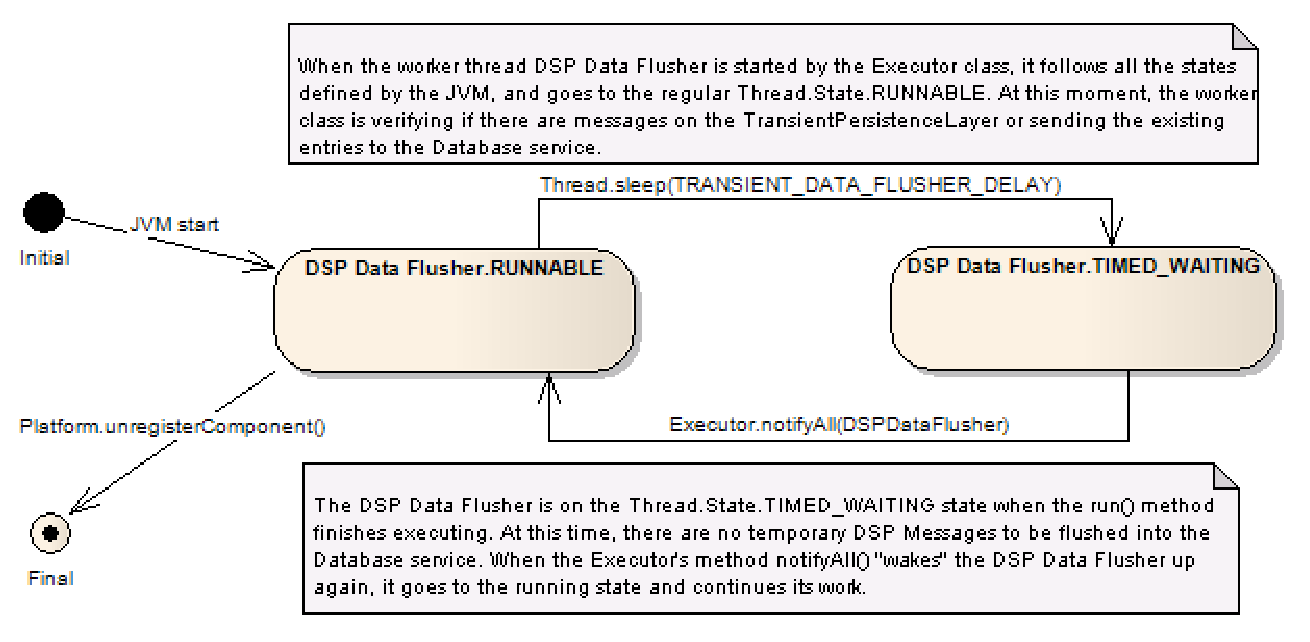
\includegraphics[scale=0.5]{../diagrams/DSP-DataPersistence-Flusher-State-Diagram}
  \caption{UML State diagram for the DSP Data Flusher Worker Thread}
  \label{fig:DSP-DataPersistence-Flusher-State-Diagram}
\end{figure}

Upon receiving a new DSP measurement message, the DSP Data Persistence
component must send its reference to the temporary memory space, as described
by the non-functional requirement on section 3.2. In this way, the DSP Data
Persistence component maintains a dependency on the Singleton class
TransientPersistenceLayer, which is responsible for keeping track of messages
that are received by working component. However, in order to add the DSP
message into its aggregated map, it first transforms the message into an
instance of the class PersistentMessageUnit, which has references to the class
regarding the location of the message,  SensorLocation.

The last paragraph of section 2.4.7 described the last steps of the Sequence
Diagram regarding DSP Message delivery to the DSP Broker on the DSP Server
host. For this reason, Image 3.4.1.2 continues the steps of the DSP Broker from
the gate "From DSP WireTransport Server to Broker Gate", showing the steps
taken to transfer a DSP Message to the Singleton class
TransientPersistenceLayer.

According to the DSP Broker model described on section 2.4.6, the DSP Matcher
needs to be updated with the addition of a matching rule that filters a copy of
any Measurement Message (section 2.4.4) to the DSP Data Persistence component
designed. As it is shown in figure
\ref{fig:From-DSP-Broker-To-DSPDataPersistence-General-Sequence}, the worker
Thread DSP Data Flusher is the link between the Transient and Persistent
layers, as it depends on the references from the classes
TransientPersistenceLayer and the DSPMongoCRUDService. The former maintains
DSP Messages in memory wrapped by an instance of PersistenceMessageUnit and
the latter is responsible for sending the MessageContent from the DSPMessage
body to the Database.

\begin{figure}[!b]
  \centering
  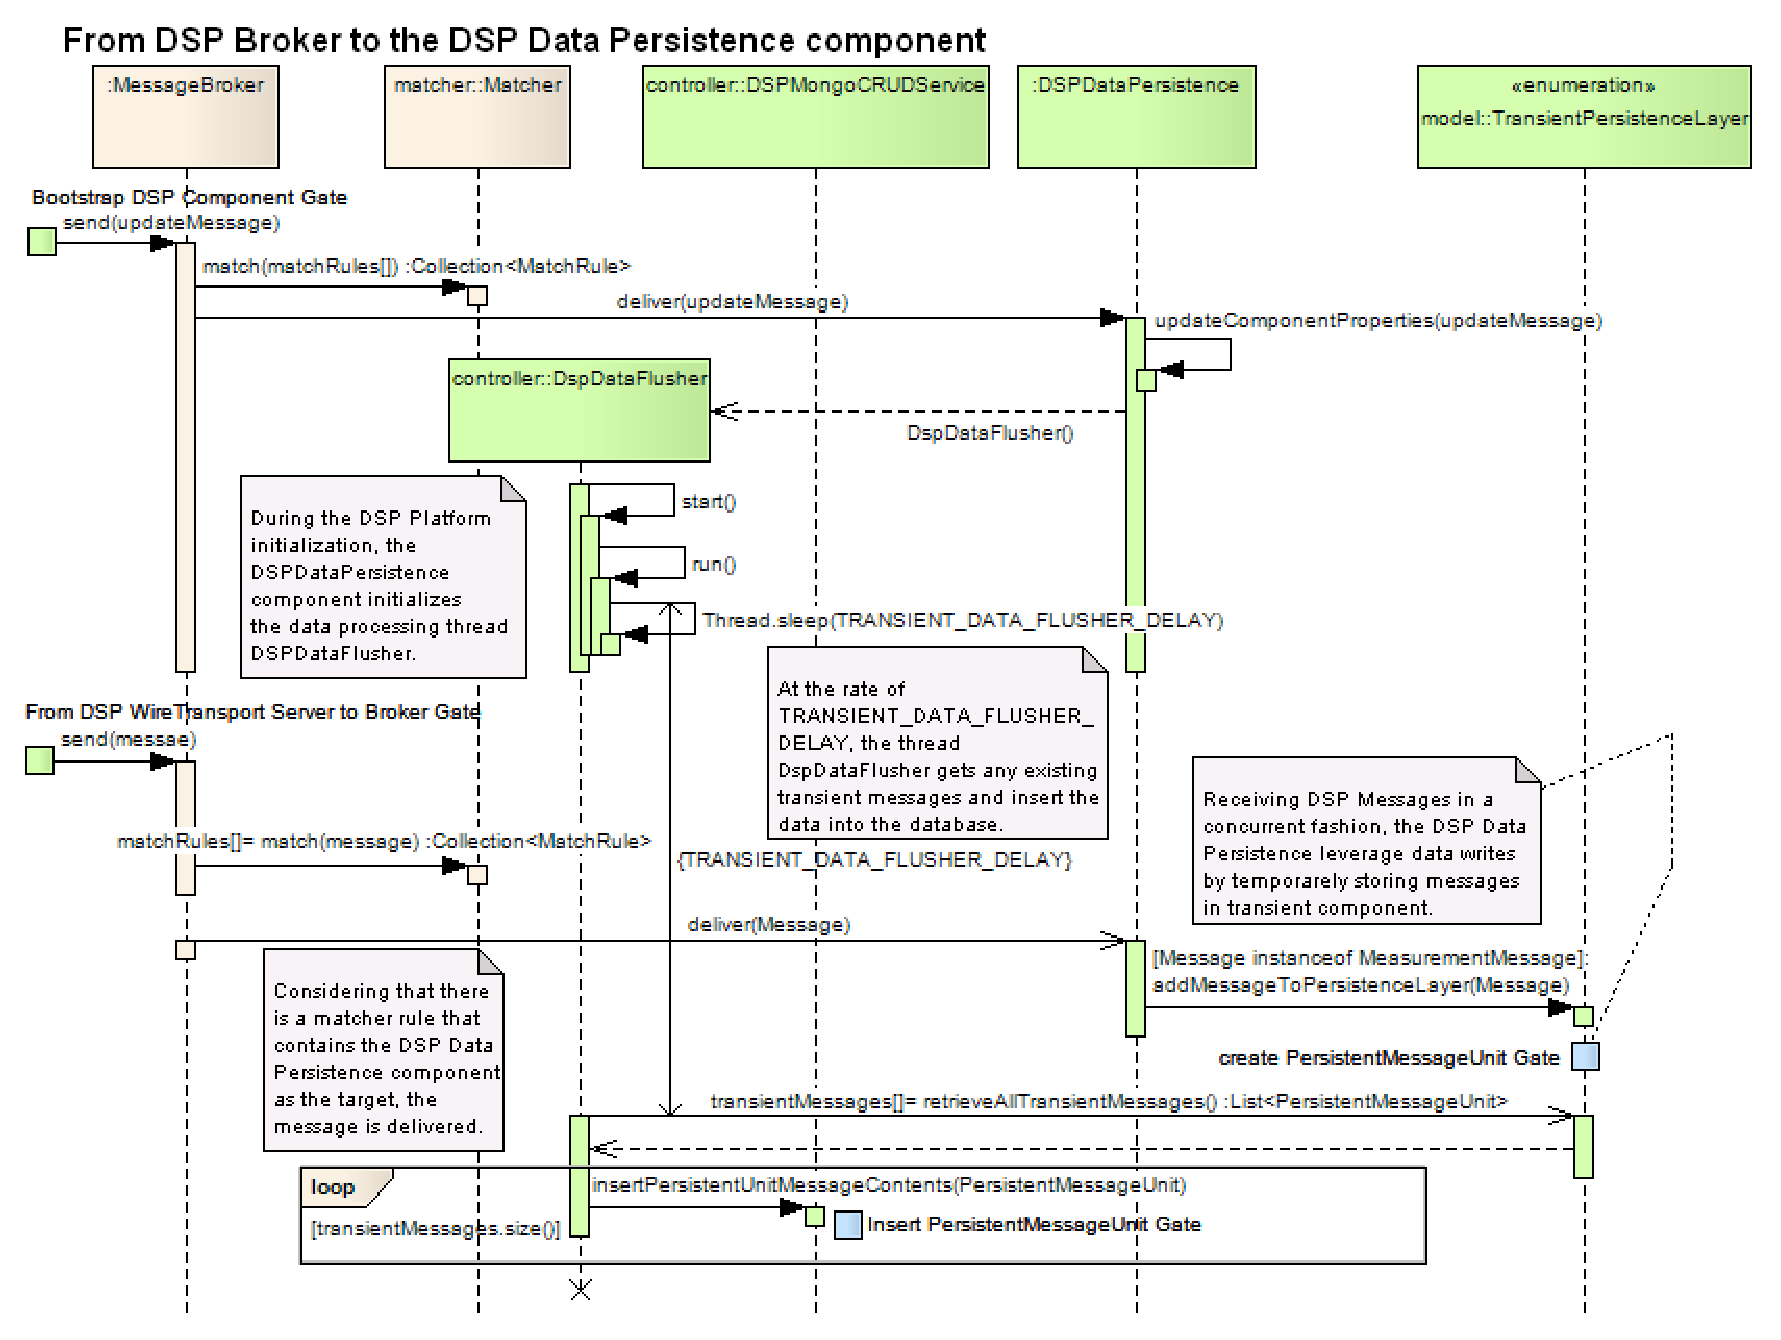
\includegraphics[scale=0.5]{../diagrams/From-DSP-Broker-To-DSPDataPersistence-General-Sequence}
  \caption{UML Sequence Diagram - Flow 1: From the DSP Broker to the Data
  Persistence Component}
  \label{fig:From-DSP-Broker-To-DSPDataPersistence-General-Sequence}
\end{figure}

The DSP Broker retrieves the list of matching rules by contacting the Matcher.
As the DSP Platform have already loaded all the Matching rules, a copy of a
given DSP message is delivered to the DSP Data Persistence component. However,
the sequence diagram shows two different stages of reception:

\begin{itemize}
  \item A bootstrap DSP Update Message is delivered to the DSP Data Persistence
  component when the DSP Platform is initializing the component. In this way,
  the DSP Data Persistence can initialize the DspDataFlusher worker thread to
  flush temporary messages into the database at the rate of
  TRANSIENT\underline{ }DATA\underline{ }FLUSHER\underline{ }DELAY in seconds;
  \item Any DSP Measure Message can be persisted by the DSP Data Persistence
  component. When the DSP Broker delivers a DSP MeasureMessage to this
  component, it will add the message to a temporary memory location to decrease
  I/O on the database, as depicted by the gate "create PersistentMessageUnit
  Gate". The simple procedure to add the message into the transient persistent
  layer is shown on image 3.4.3.
\end{itemize}

The class PersistenceMessageUnit is the major transient persistence unit that
carries references regarding the originating DSP Message that was collected by
the DSP Data Persistence component. It is composed by a SensorLocation and
contains a reference to the PersistentMessageState enumaration. The former
identifies which sensor produced the collected data from the DSP Message by the
IP address, while the latter identifies whether the PersistenceMessageUnit has
been saved into the Database or not as depicted by the UML State diagram in
figure \ref{fig:PersistentMessageState-Diagram}.

\begin{figure}[!b]
  \centering
  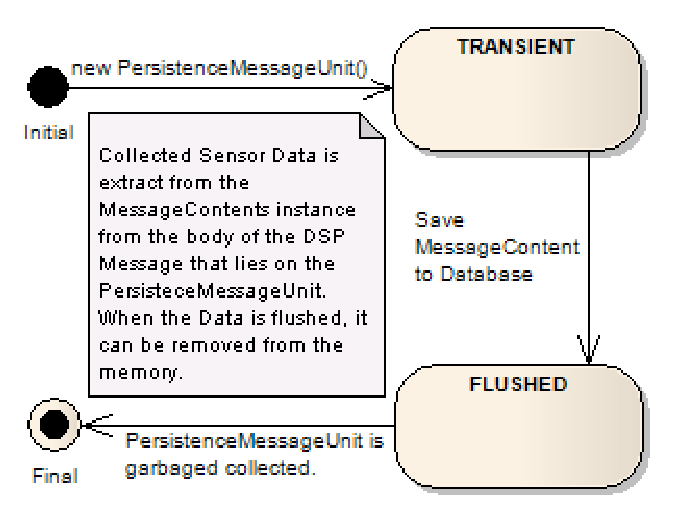
\includegraphics[scale=0.5]{../diagrams/PersistentMessageState-Diagram}
  \caption{UML State Diagram for the instance of the class
  PersistentMessageState}
  \label{fig:PersistentMessageState-Diagram}
\end{figure}

\begin{figure}[!b]
  \centering
  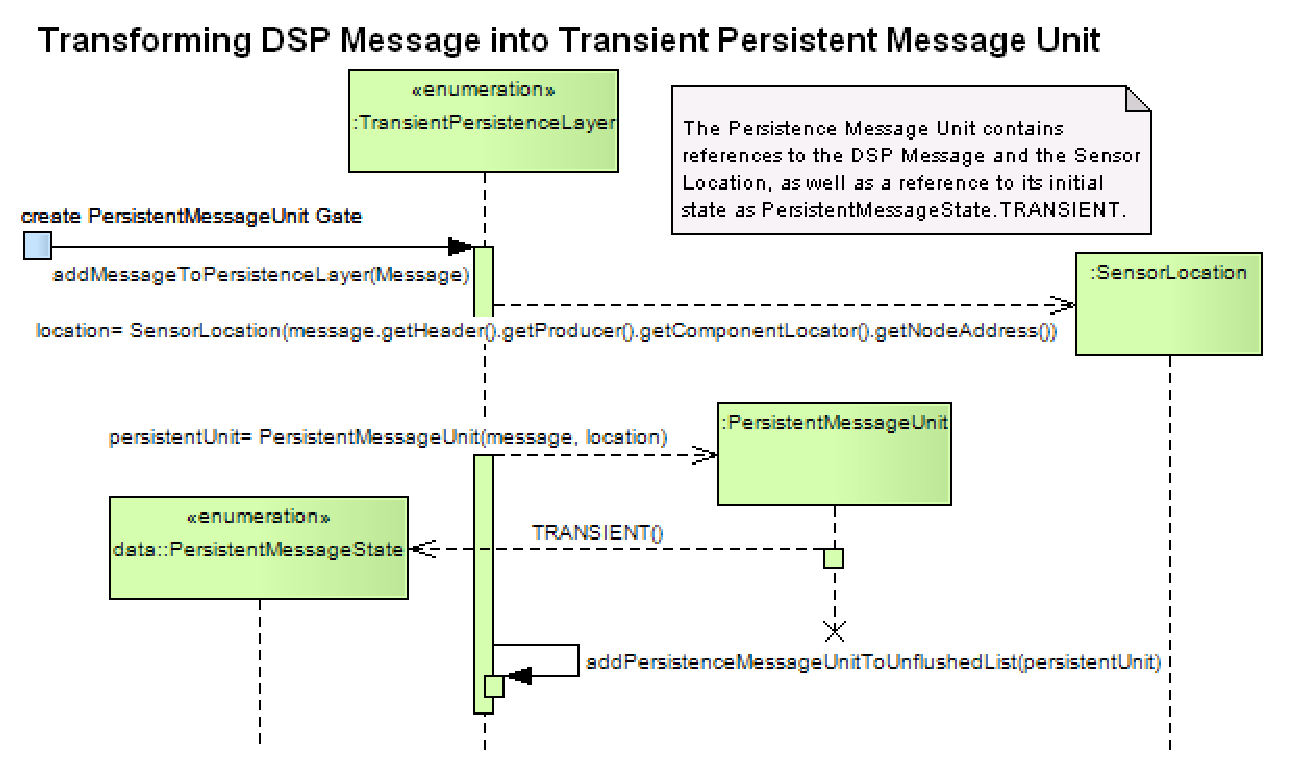
\includegraphics[scale=0.5]{../diagrams/From-Create-PersistentMessageUnit-to-TransientPersistence-Layer-Sequence}
  \caption{UML Sequence diagram - Adding a DSP Message into the Transient Persistence layer}
  \label{fig:From-Create-PersistentMessageUnit-to-TransientPersistence-Layer-Sequence}
\end{figure}

According to section 3.4.1, the persistence model must carry information
regarding which sensor device produced the collected data. For this reason, an
instance of the class SensorLocation carries the information about the IP
address from the component that originally produced the DSP Message. Then, an
instance of the class PersistenceMessageUnit is created, having its state on
TRANSIENT, as detailed on UML State diagram on Image 3.4.2.

\subsection{Flushing data into the Database}

The last stage sequence described on the Sequence diagram of Image 3.4.3
depicts the DspDataFlusher worker thread continuously waking up at the rate of
TRANSIENT\underline{ }DATA\underline{ }FLUSHER\underline{ }DELAY. Its purpose is as simple as to iterate over the
list of PersitenceMessageUnit on the state of TRANSIENT, and send each of them
to be saved on the persistence storage. Figure
\ref{fig:DSP-Data-Persistence-Classes} shows the participating classes of the
component.

\begin{figure}[!b]
  \centering
  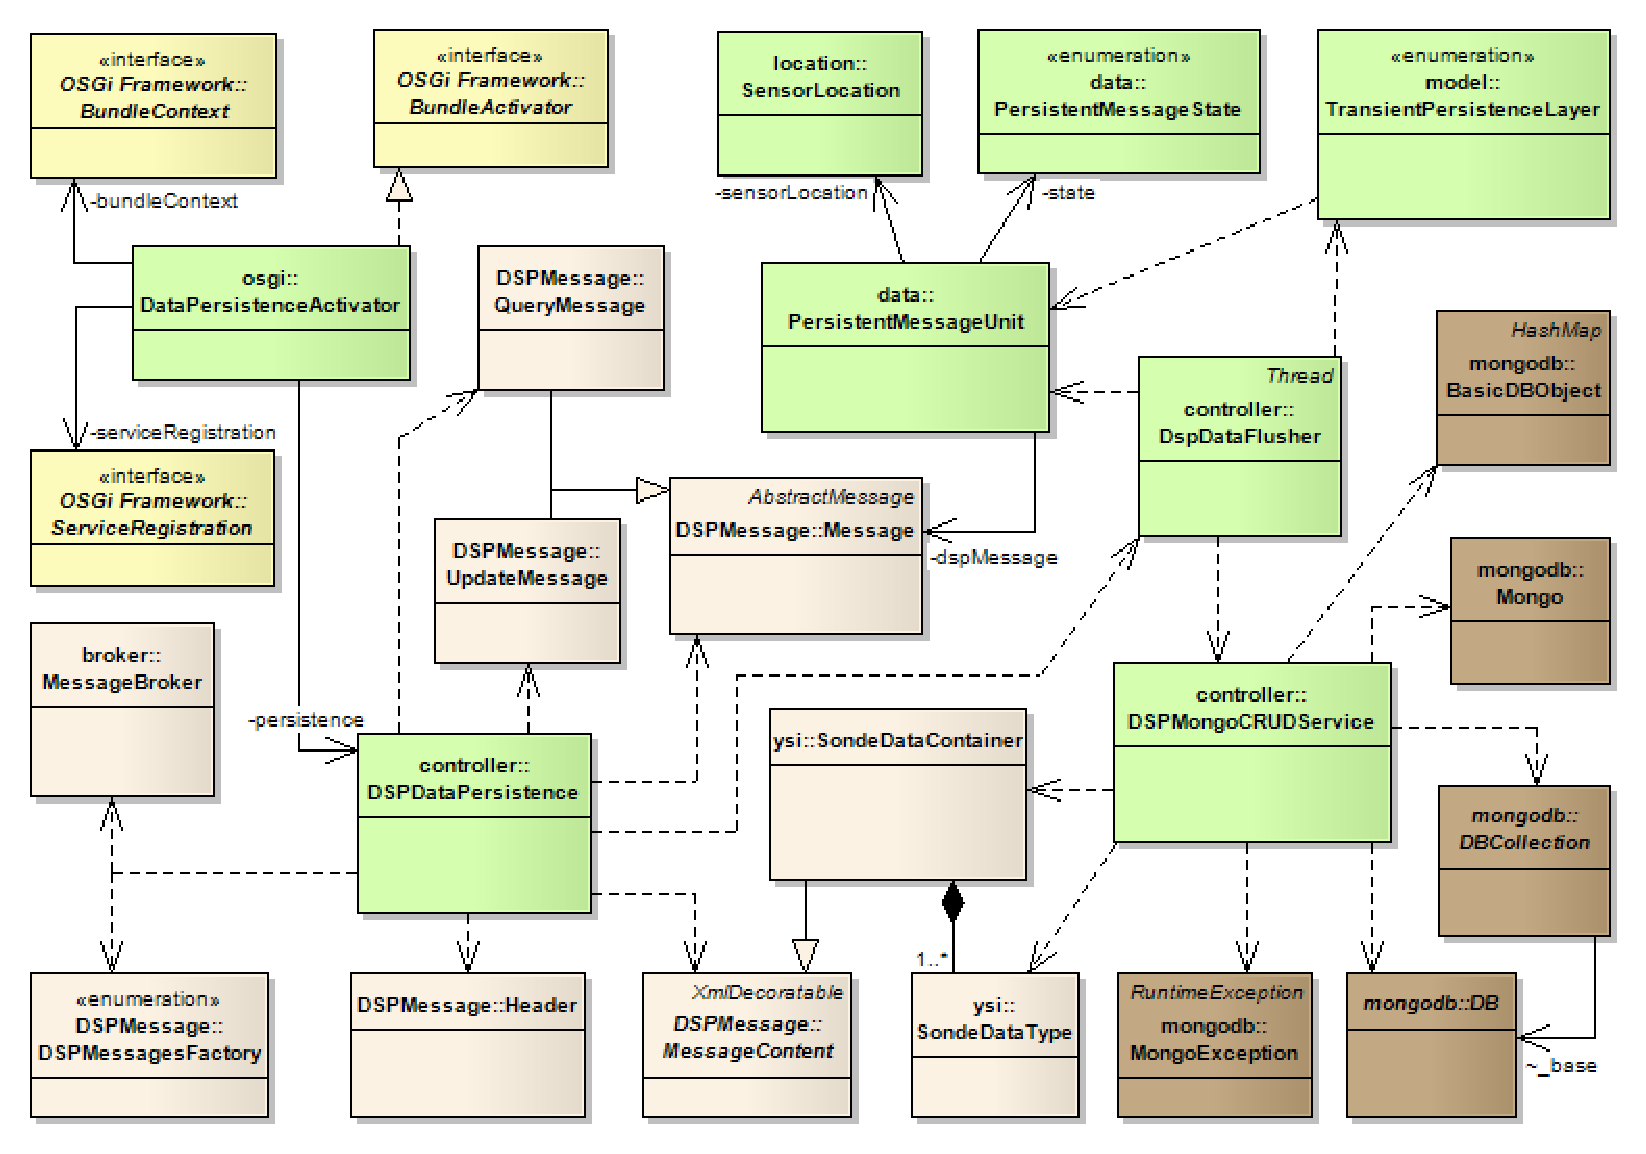
\includegraphics[scale=0.5]{../diagrams/DSP-Data-Persistence-Classes}
  \caption{UML Class diagram for the DSP Data Persistence component.}
  \label{fig:DSP-Data-Persistence-Classes}
\end{figure}

Finally, this sequence of events is continued by the "insert
PersistenceMessageUnit Gate", which triggers the persistence service from the
chosen database system as shown on Image 3.4.5.

\begin{figure}[!b]
  \centering
  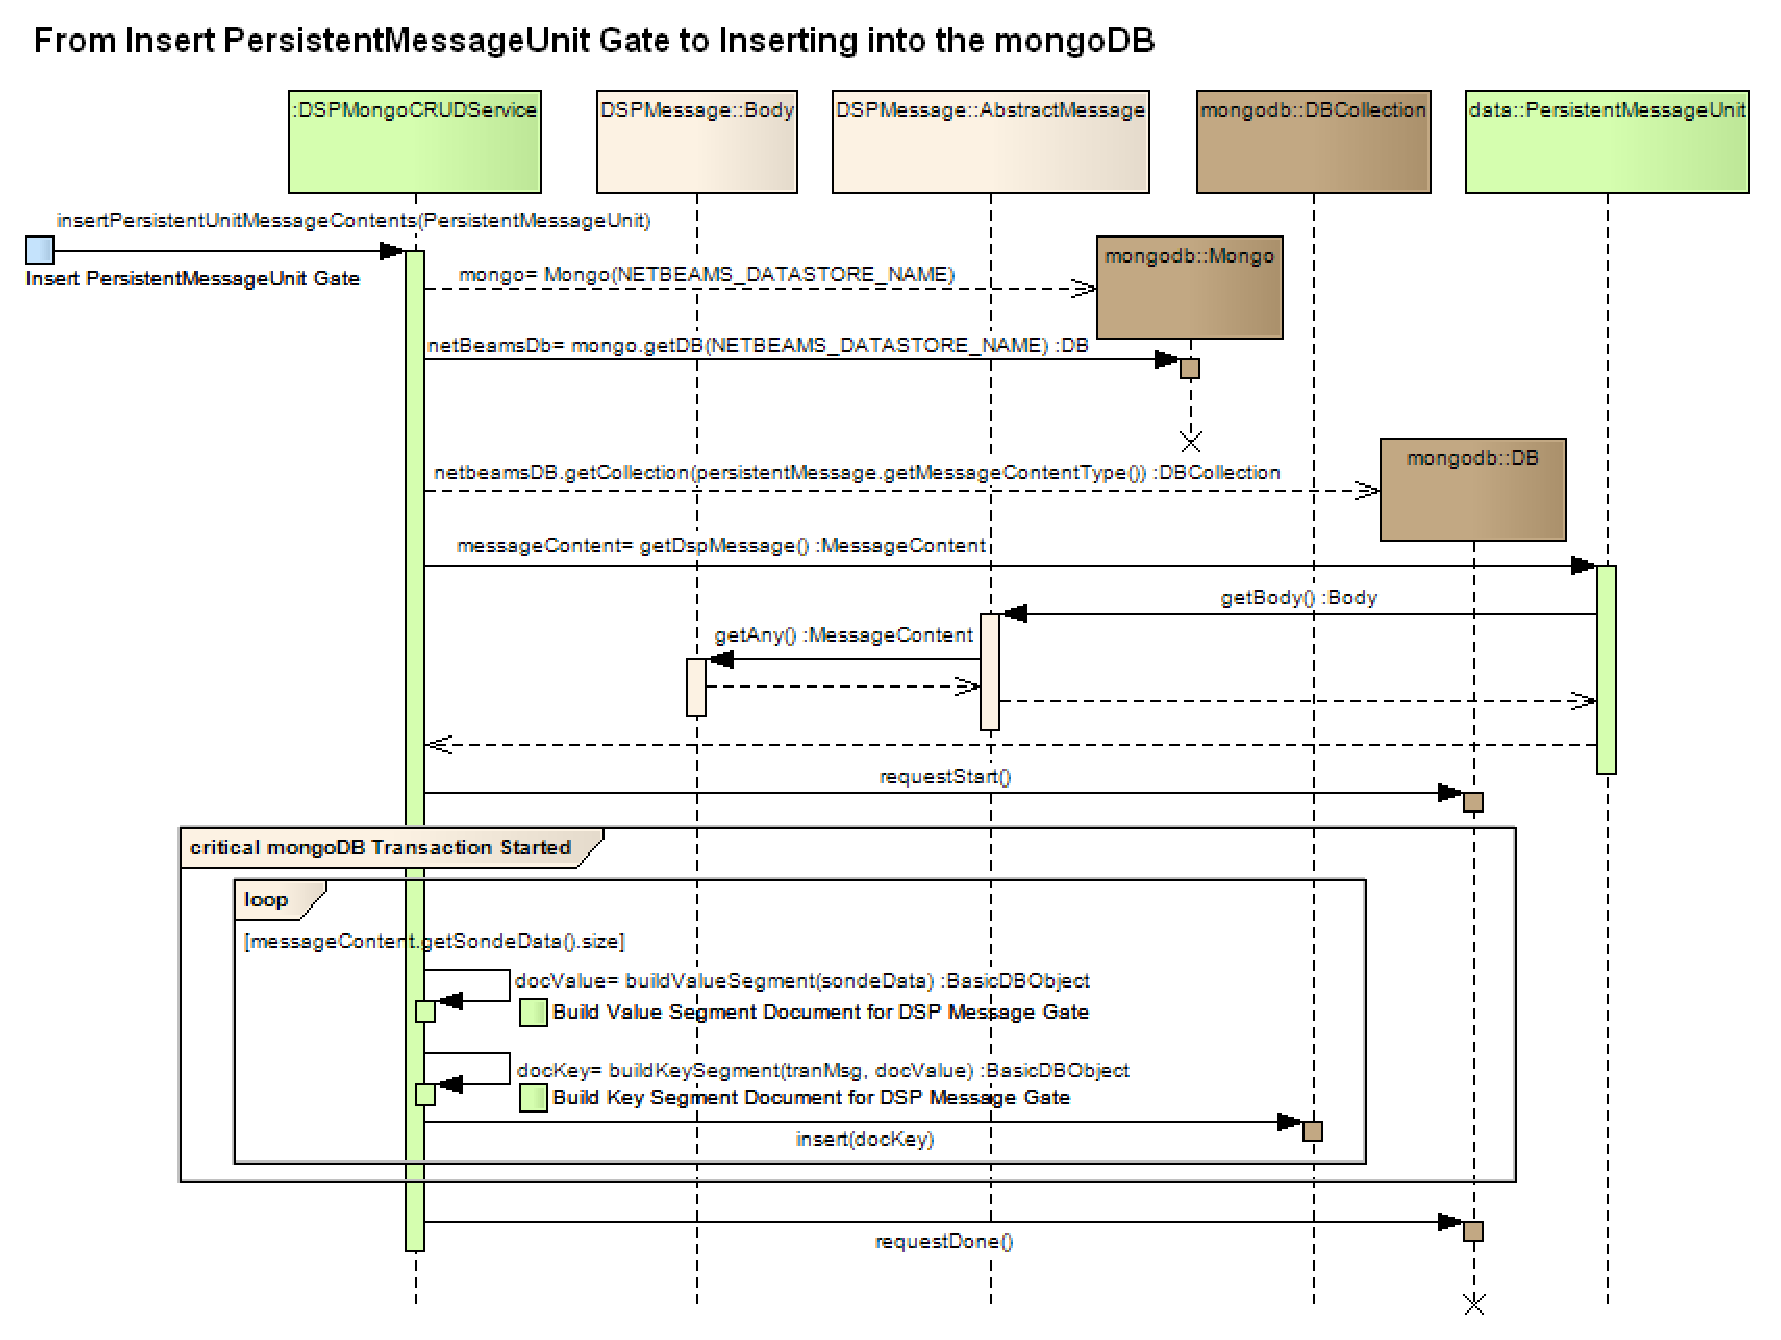
\includegraphics[scale=0.5]{../diagrams/From-Insert-PersistentMessageUnit-to-mongoDB}
  \caption{UML Sequence Diagram - MessageContent instance saved by the class
  mongoDB service}
  \label{fig:From-Insert-PersistentMessageUnit-to-mongoDB}
\end{figure}

In order to build the document key and value segments as described on section
3.2. First, the value is built by extracting the DSP Message Content from the
body of the DSP Message.

\begin{figure}[!b]
  \centering
  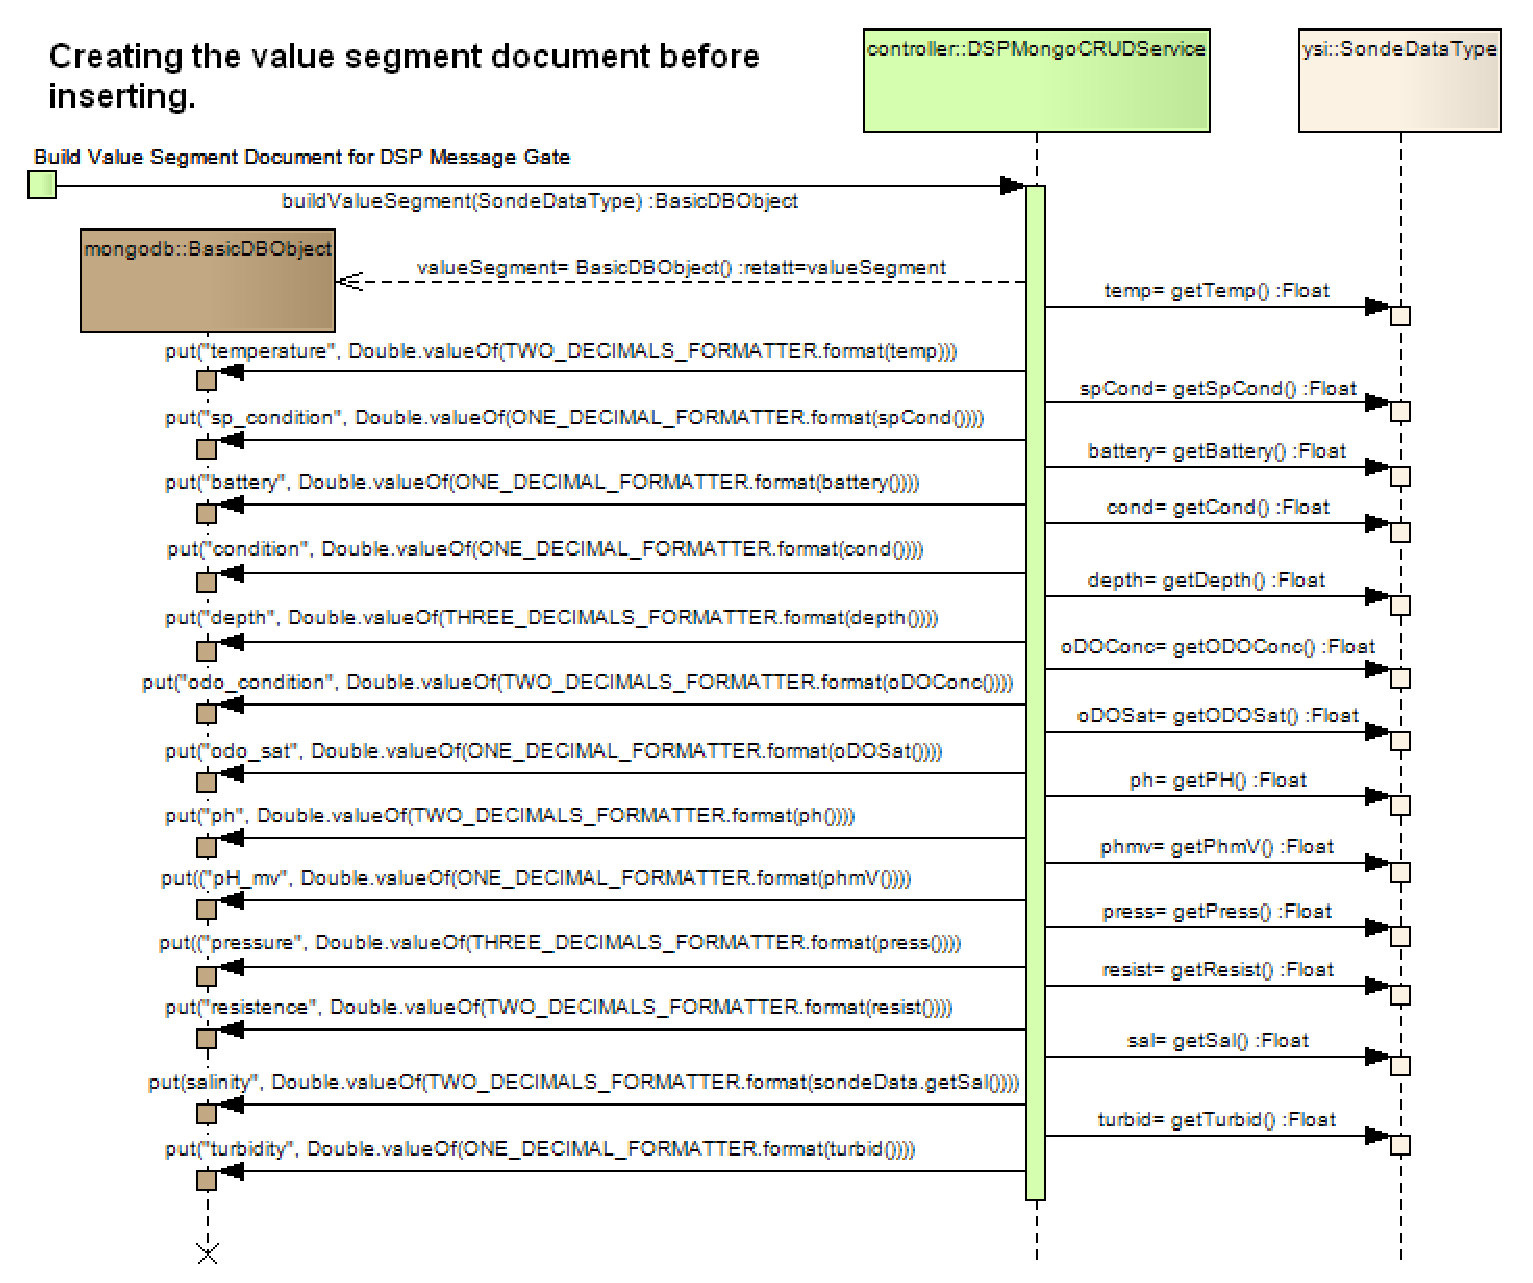
\includegraphics[scale=0.5]{../diagrams/From-Creating-Value-Segment-Sequence}
  \caption{UML Sequence diagram showing the creation of the value document segment}
  \label{fig:From-Creating-Value-Segment-Sequence}
\end{figure}

Finally, the document key segment is prepared as follows on image 3.4.7.

\begin{figure}[!b]
  \centering
  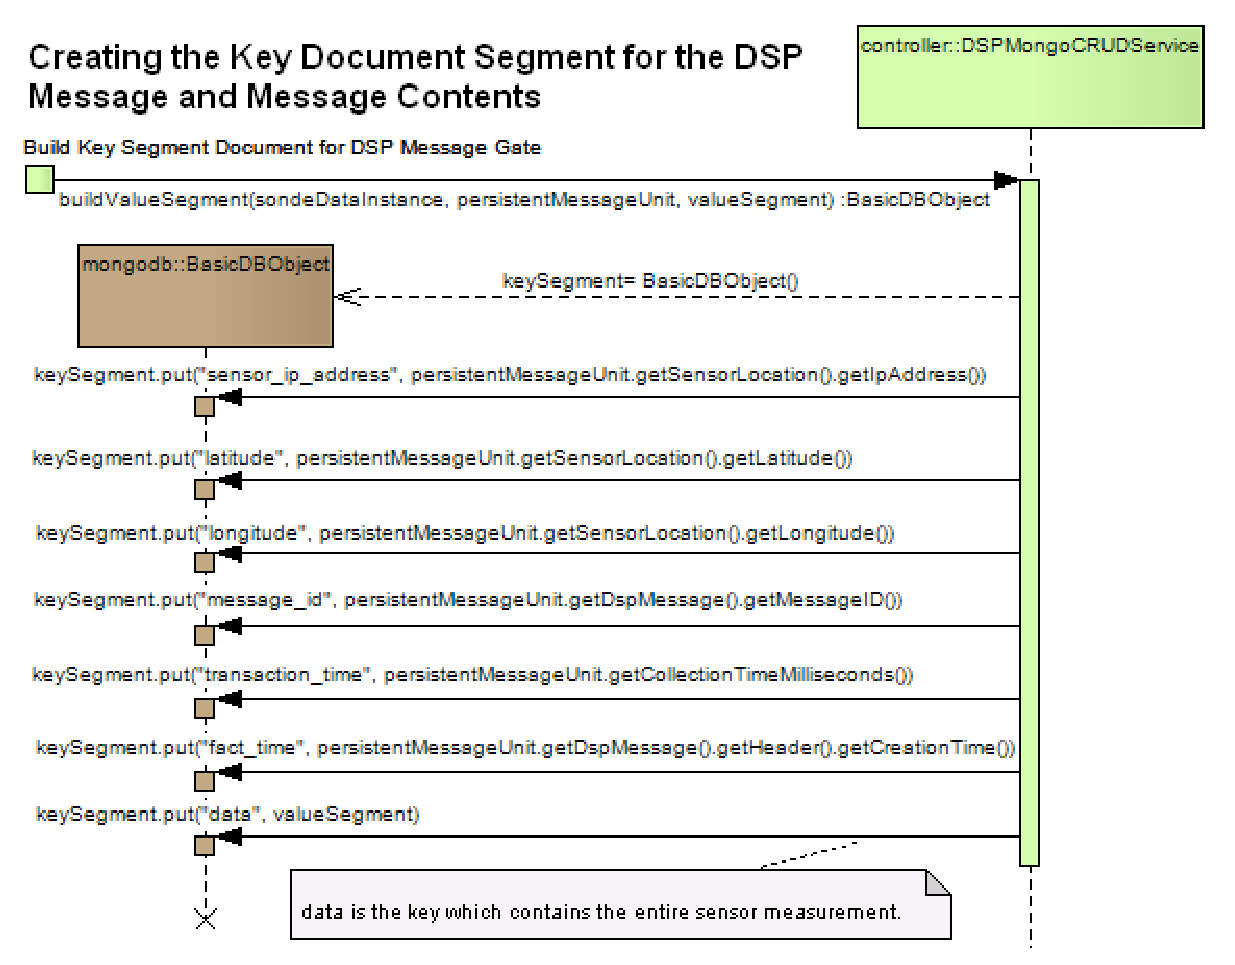
\includegraphics[scale=0.5]{../diagrams/From-Creating-Key-Segment-Sequence}
  \caption{UML Sequence diagram showing the creation of the key document segment}
  \label{fig:From-Creating-Key-Segment-Sequence}
\end{figure}







\subsection{DSP Data Persistence Implementation}

This section shows the implementation of the DSP Data Persistence, which
follows the specifications of the DSP Components described on section 2.4,
along with the setup of the mongoDB, the chosen database system that handles
document-oriented instances. The implementation of the DSP Data Persistence
component was developed using the DSP Subversion repository at
http://code.google.com/p/netbeams.

The Deployment diagram with a single host, single database;
Deployment diagram with single host, multiple shards;
Deployment diagram with dedicated database host, single database;
Deployment diagram with dedicated cluster host, multiple shards/replicas;

Each of the deployment schema have two different deployment components: the DSP
component deployment and the database instance installation and configuration.
The following section shows each of the components artifacts and configuration
necessary.

\subsubsection{DSP Deployment on OSGi Framework}

    * Description of the OSGi MANIFEST.MF
    * Description of the component on the config.xml
    * Adding a matching rule on the matcher\underline{ }config.xml
    * Adding a bootstrap message the component and database configuration


    * Adding a new entry into the deployment configuration artifact config.xml;
    * Adding a new entry into the matcher configuration artifact matcher\underline{ }config.xml;
    * Adding an optional configuration message that sets up the new DSP Component;
    * Adding new Java drivers that communicates with the Database system;
    * Installing and configuring the proposed database system.